\subsection*{Case 7} % smartly california (viralspace.ai)
\label{case: 7}

% Inference architecture
% \begin{figure*}[t]
% \centering
% 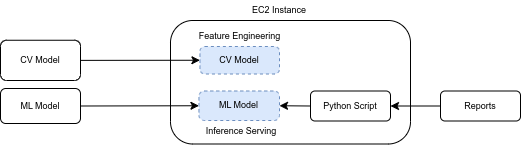
\includegraphics[width=0.8\textwidth]{images/case7_deployment_process_v2.png}
% \caption{Case 7 deployment setup}
% \label{fig: case7_deployment_process}
% \end{figure*}

% Inference architecture
\begin{figure*}[t]
\centering
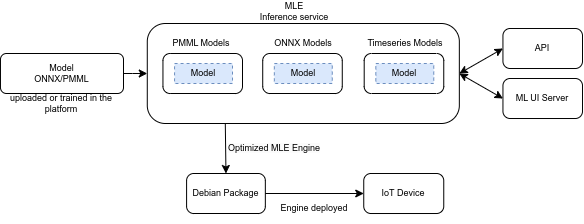
\includegraphics[width=0.9\textwidth]{images/case6_deployment_process_v2.png}
\caption{Case 6 Inference Architecture}
\label{fig: case6_deployment_process}
\end{figure*}

The case company offers a machine learning (ML) system that generates targeted digital advertisements by optimizing the creative elements of ads and suggesting features that can enhance a brand's marketing campaign. The system can also be used to predict an advert's performance before the start of a campaign. The ML solution is comprised of two ML subsystems: i) a computer vision model used for feature engineering tasks such as extracting features from image or video data and performing tagging and labelling, ii) an ML model (non-neural network) that is trained using the features extracted by the CV model. The second model is employed to draw inferences for the business case. These ML models are used internally to generate non-technical reports. As such, customers do not interact with the models directly. % by estimating key performance metrics such as cost per acquisition.

\textit{Pre-Integration}: Generally, the infrastructure is based on AWS services. EC2 instances are used to perform training and inference tasks, while S3 buckets are used to store trained models. The deployment workflow is manually orchestrated. Various elements in the workflow are orchestrated through Python scripts and manual interventions. Each customer is associated with a dedicated model, and the operation's scale involves tens of models, adding to the pipelines' complexity and the general workflows.

Active models are retrained daily to ensure the model accounts for new data obtained from the campaigns. This involves about 100MBs – 1GB of new data depending on the marketing campaign size. The CV model is retrained monthly since it only extracts features from videos and images. The versioning of the models is based on the S3 storage policy, which works as the model retirement policy.

\textit{Quality assurance}: The quality assurance process is centered around a human-in-the-loop workflow. Before deployment, a human reviewer locally validates the performance of a new model to ensure that it meets the required metrics, such as F1-score, or ensures the accuracy of the CV model used for tagging and labelling images is acceptable.

Various factors trigger the model's retraining: new incoming data, new labels from clients for a particular feature, or new Ads being pushed by customers previously unseen by the models.

\textit{Server Environment}: The models and related runtime dependencies to the models are installed into an EC2 instance. No wrapping containers or virtual machines are used in this setting. Instead, Python scripts load models into the instance's memory and from where other components access the models.

The EC2 instance runtime is configured using bash script templates, and the same scripts can be used to create a local runtime environment for development purposes. The runtimes can be used for inference machines or other data exploration tasks. Although the environment is not containerized, the scripts provide a flexible template for managing the runtime environment and adapting it to various needs in the workflow.

\textit{Inference}: The inference pipeline is automated using AWS Lambda. The model object is loaded into the instance's memory, and batch inference is conducted using a Python script. The inference results are then persisted in a database for subsequent report generation. Lambda execution environment offers automatic scaling capabilities which support inference across multiple models and in a single model. Figure~\ref{fig: case7_deployment_process} presents an architectural view of this setup.

Inference for the CV model is used as part of feature engineering and data pre-processing. Pre-processing tasks such as tagging, labelling, encoding strings, and converting them into a vector space are conducted with the CV model.

\textit{Monitoring}: Monitoring begins with ensuring the model's availability using the AWS CloudWatch service. However, logging is the primary method for collecting lower-level information about processes and system events. Other tools such as Lambda, Slack, Email, and Pager Duty are integrated into the monitoring workflow to process events and logs. Given the complex nature of the system, which comprises multiple models, monitoring can become challenging, particularly with the diversity of alerts generated across various channels.

% Inference architecture
\begin{figure*}[ht!]
\centering
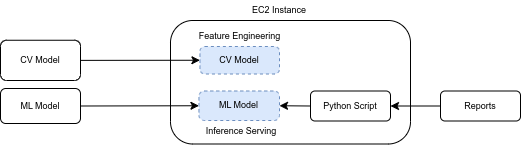
\includegraphics[width=0.8\textwidth]{images/case7_deployment_process_v2.png}
\caption{Case 7 Inference Architecture}
\label{fig: case7_deployment_process}
\end{figure*}
